\chapter{Disseny i construcció del sistema}
\label{chap:construccio}

\section{Introducció}
\label{sec:introduccio}

Aquest document descriu el disseny, la construcció i la validació en vol d'un sistema complet d'aerofotogrametria de precisió (\emph{surveying} amb dron): una base GNSS RTK pròpia, un UAV amb doble receptor GNSS i una càmera amb sincronisme de sabata, i una estació de terra que els enllaça.

L'objectiu és aconseguir geoetiquetat centimètric de les fotografies aèries ($\leq 2$~cm en horitzontal, $\leq 3$~cm en vertical) per generar ortomosaics i models digitals de superfície de qualitat topogràfica, amb un cost total de maquinari al voltant dels 2.150~€ --~una fracció del cost d'un DJI P4 RTK o d'un conjunt Emlid~+~UAV~-- i amb control total sobre el \emph{firmware}, les correccions i el flux de dades.

El sistema es divideix en tres subsistemes:
\begin{itemize}
    \item \textbf{Base GNSS RTK}: estació fixa que genera correccions RTCM3.
    \item \textbf{UAV (\emph{rover})}: dron amb doble receptor GNSS per a posicionament RTK i \emph{heading} per \emph{moving baseline}.
    \item \textbf{Estació de terra (GS)}: enllaç de telemetria i redistribució de correccions cap al dron.
\end{itemize}

El document s'organitza en quatre blocs: el disseny i la construcció (aquest capítol), el manual d'operació i procediments (\cref{chap:manual}), la campanya de proves de vol i posada a punt (\cref{chap:proves-vol}) i els vols de fotogrametria que en resulten (\cref{chap:vols-prova}).

\section{Arquitectura i flux de dades}
\label{sec:arquitectura}

L'arquitectura escollida fa servir la base per servir correccions RTCM3 per WiFi local (mode \emph{access point}) mitjançant un servidor TCP propi, sense NTRIP. Es va descartar l'enllaç ràdio directe base~$\rightarrow$~dron per simplificar el sistema (un sol canal de ràdio al dron) i per guanyar resiliència en zones rurals sense cobertura mòbil.

\begin{figure}[H]
    \centering
    \resizebox{\linewidth}{!}{%
    \begin{tikzpicture}[
        box/.style={draw, rounded corners=2pt, align=center, font=\small, minimum height=10mm, minimum width=27mm, fill=blue!5},
        arr/.style={-{Stealth[length=2mm]}, thick},
        grp/.style={draw, dashed, rounded corners=4pt, inner sep=4mm, gray},
        node distance=8mm and 17mm]
        \node[box] (ant) {Antena\\multibanda};
        \node[box, right=of ant] (f9b) {ZED-F9P\\(base, \emph{survey-in})};
        \node[box, right=of f9b] (pi) {Raspberry Pi\\servidor TCP};
        \node[box, below=16mm of pi] (gs) {Mission Planner\\(estació de terra)};
        \node[box, left=of gs] (rfdg) {RFD868x\\(costat GS)};
        \node[box, below=16mm of rfdg] (rfdu) {RFD868x\\(costat dron)};
        \node[box, right=of rfdu] (fc) {Controlador de vol\\(Kakute H7, EKF3)};
        \node[box, right=of fc] (gnss) {2$\times$ ZED-F9P\\\emph{moving baseline}};
        \node[box, below=10mm of fc] (cam) {Sony $\alpha$6000\\MAP2 + SYNC2};
        \draw[arr] (ant) -- (f9b);
        \draw[arr] (f9b) -- node[above, font=\scriptsize] {RTCM3} (pi);
        \draw[arr] (pi) -- node[right, font=\scriptsize] {WiFi} (gs);
        \draw[arr] (gs) -- node[above, font=\scriptsize] {USB} (rfdg);
        \draw[arr] (rfdg) -- node[right, font=\scriptsize] {868~MHz} (rfdu);
        \draw[arr] (rfdu) -- node[above, font=\scriptsize] {MAVLink} (fc);
        \draw[arr, <->] (fc) -- node[above, font=\scriptsize] {UART} (gnss);
        \draw[arr, <->] (fc) -- node[right, font=\scriptsize] {PWM / sabata} (cam);
        \begin{scope}[on background layer]
            \node[grp, fit=(ant)(f9b)(pi), label={[font=\small, gray]above:Base RTK}] {};
            \node[grp, fit=(rfdu)(fc)(gnss)(cam), label={[font=\small, gray]above:UAV}] {};
        \end{scope}
    \end{tikzpicture}}
    \caption{Diagrama de blocs del sistema i flux de les correccions RTCM3.}
    \label{fig:diagrama-blocs}
\end{figure}

\subsection{Flux complet de dades}

\begin{enumerate}[label=\arabic*.]
    \item L'antena multibanda capta L1/L2/L5 (GPS, GLONASS, Galileo, BeiDou).
    \item El \textbf{ZED-F9P} de la base (mode \emph{survey-in} a cada sessió, \cref{sec:protocol-camp}) genera missatges \textbf{RTCM3} (1005, 1074, 1084, 1094, 1124 i 1230) a 1~Hz. El 1005, amb la posició de la base, només surt quan el \emph{survey-in} és vàlid.
    \item La \textbf{Raspberry Pi} rep aquests missatges per USB (port sèrie del receptor simpleRTK2B Pro) i els redistribueix tal com arriben pel servidor TCP del port 5000, per WiFi AP.
    \item La \textbf{GS} (Mission Planner / QGroundControl al costat del pilot) es connecta al servidor TCP i reenvia el flux RTCM3 al dron per MAVLink (\texttt{GPS\_RTCM\_DATA}) a través del parell \textbf{RFD868x}.
    \item Al dron, el F9P primari rep les correccions, calcula la posició RTK i, en mode \emph{moving baseline}, genera RTCM 4072.x cap al secundari per derivar el \emph{heading}.
    \item El \textbf{FC} integra la posició RTK i el \emph{yaw} GNSS a l'EKF3 per a navegació i geoetiquetat.
\end{enumerate}

\section{Decisions de disseny}
\label{sec:decisions}

\begin{description}
    \item[Moving baseline amb 2$\times$ ZED-F9P] en lloc d'un UM982 amb \emph{heading} natiu. El F9P està més documentat, té més suport comunitari i és intercanviable entre base i UAV. Proporciona GPS-for-yaw, cosa que permet prescindir de la brúixola magnètica --~avantatge important en \emph{frames} amb molt corrent.
    \item[RFD868x per a l'enllaç GS$\leftrightarrow$UAV] als 868~MHz (banda europea) permet fins a 500~mW EIRP i un abast superior a 40~km. Sempre versió europea 868 (mai 915 o 433).
    \item[Servidor TCP local per WiFi] robust en absència de cobertura mòbil; a la pràctica gairebé sempre s'opera en local (aparcar el vehicle, muntar el trípode al costat i volar).
    \item[Retroalimentació de la sabata (Seagull SYNC2)] resol la latència variable de l'obturador ($\sim$100~ms equivalen a 1,5~m d'error a 15~m/s). Sense aquest \emph{feedback} no hi ha precisió centimètrica real al geoetiquetat; \cref{sec:retard-obturador} en quantifica l'efecte.
    \item[Post-procés PPK opcional] enregistrament de dades \texttt{UBX} en brut a la base i al dron, que permet obtenir una solució independent de la qualitat de l'enllaç RTK en temps real.
\end{description}

\section{Llista de materials}
\label{sec:materials}

El maquinari del sistema suposa un cost total de 2150~€.

\subsection{Dron}

\begin{table}[H]
    \centering
    \caption{Components del dron (UAV/\emph{rover})}
    \label{tab:materials-dron}
    \begin{tabular}{lll}
        \toprule
        Component & Model & Cost aprox. \\
        \midrule
        \emph{Frame} & S500 (Quad X, 500~mm entre eixos) & 35~€ \\
        Motors (4$\times$) & Pilotix 2808, 1100~KV & 60~€ \\
        ESC & Hobbywing XRotor 65A 4-in-1 (DShot) & 30~€ \\
        FC & Holybro Kakute H7 (STM32H7) & 55~€ \\
        GPS (2$\times$) & Holybro H-RTK F9P Helical & 510~€ (255~€/u) \\
        Telemetria & RFD868x EU 500~mW (parell dron + GS) & 363~€ \\
        RC & Radiomaster XR1 Nano ELRS dual-band & 16~€ \\
        Bateria & Gaoneng GNB 6S 4000~mAh 70C & 70~€ \\
        \bottomrule
    \end{tabular}
\end{table}

\begin{description}
    \item[Motors Pilotix 2808, 1100~KV] KV moderat per a 6S, pensat per a hèlixs de 8~polzades (\cref{tab:kv-compatibilitat}) amb la càrrega útil addicional del sistema RTK~+~càmera, en lloc dels KV alts típics de \emph{freestyle}, que sacrifiquen eficiència per velocitat. Les hèlixs de 7~polzades del muntatge inicial van ser per disponibilitat, no per disseny (\cref{subsec:propulsor-inicial}).
    \item[ESC Hobbywing XRotor 65A 4-in-1 (DShot)] marge de corrent per al pes addicional; el DShot bidireccional permet telemetria de RPM per motor, útil per a diagnòstic de vibracions; el format 4-in-1 simplifica el cablejat de potència.
    \item[FC Holybro Kakute H7 (STM32H7)] prou ports UART per a tota l'arquitectura sense necessitat d'expansió (2$\times$F9P, RFD868x, RC ELRS, telemetria ESC, USB) i suport natiu a ArduPilot per a GPS \emph{moving baseline} i DShot.
    \item[GPS Holybro H-RTK F9P Helical (2$\times$)] mòdul integrat (antena helical + \emph{breakout} F9P) ja pensat per a \emph{moving baseline} amb ArduPilot; evita haver de dissenyar i aparellar antena i \emph{breakout} per separat.
    \item[Telemetria RFD868x] justificació completa a \cref{sec:decisions}.
    \item[RC Radiomaster XR1 Nano ELRS] mida i pes mínims per no penalitzar la càrrega útil; ELRS de baixa latència complementa el RFD868x, que porta les dades MAVLink/RTCM però no el control de vol.
    \item[Bateria Gaoneng 6S 4000~mAh 70C] 6S per millor eficiència de tensió amb el consum addicional (GPS, telemetria, càmera); 70C dona marge de corrent de pic suficient amb els 4 motors a plena càrrega.
\end{description}

\subsection{Base GNSS}

\begin{table}[H]
    \centering
    \caption{Components de la base RTK}
    \label{tab:materials-base}
    \begin{tabular}{lll}
        \toprule
        Component & Model & Cost aprox. \\
        \midrule
        GNSS & ArduSimple simpleRTK2B Pro (ZED-F9P) & 126~€ \\
        Antena & BD900 GNSS (multibanda) & 43~€ \\
        SBC & Raspberry Pi Zero W & 35~€ \\
        Alimentació & Waveshare UPS HAT + 2$\times$ 18650 3500~mAh & 47~€ \\
        \bottomrule
    \end{tabular}
\end{table}

\begin{description}
    \item[GNSS simpleRTK2B Pro (ZED-F9P)] placa de desenvolupament amb USB i connector d'antena SMA, amb el mateix xip que els receptors del dron, cosa que dona intercanviabilitat i una configuració i un \emph{firmware} compartits (\cref{sec:decisions}).
    \item[Antena BD900 GNSS (multibanda)] necessària per rebre les dues bandes i les múltiples constel·lacions que fa servir el ZED-F9P, requisit perquè el \emph{survey-in} convergeixi (\cref{sec:protocol-camp}).
    \item[Raspberry Pi Zero W] mida i consum reduïts per a ús en camp amb bateria, amb prou capacitat per distribuir les correccions pel servidor TCP i fer de punt d'accés WiFi (NetworkManager).
    \item[Alimentació UPS HAT + 2$\times$18650] autonomia de la base independent de la xarxa elèctrica al camp, amb protecció davant talls durant l'enregistrament.
\end{description}

\subsection{Estació de terra}

\begin{table}[H]
    \centering
    \caption{Components de l'estació de terra (GS)}
    \label{tab:materials-gs}
    \begin{tabular}{lll}
        \toprule
        Component & Model & Cost aprox. \\
        \midrule
        Comandament & Radiomaster TX16S (o similar) ELRS & 167~€ \\
        Telemetria & RFD868x (costat GS, inclòs al parell) & -- \\
        Portàtil / tauleta & Propi, amb Mission Planner & -- \\
        \bottomrule
    \end{tabular}
\end{table}

El comandament i el parell RFD868x són elements estàndard sense decisió específica de disseny. L'únic element addicional de la GS és el portàtil o la tauleta amb Mission Planner o QGroundControl, que fa de pont entre el servidor TCP de la base i el flux MAVLink cap al dron (\cref{sec:arquitectura}).

\subsection{Càmera (mòdul de cartografia)}

\begin{table}[H]
    \centering
    \caption{Mòdul de càmera per a fotogrametria}
    \label{tab:materials-camera}
    \begin{tabular}{lll}
        \toprule
        Component & Model & Cost aprox. \\
        \midrule
        Cos & Sony $\alpha$6000 (24~MP APS-C, segona mà) & 200~€ \\
        Òptica & TTArtisan 25~mm f/2 APS-C, enfocament manual & 71~€ \\
        \emph{Trigger} & Seagull MAP2 (dispar per PWM) & 30~€ \\
        \emph{Feedback} & Seagull SYNC2 (sabata, X-sync $\rightarrow$ FC) & 30~€ \\
        Targeta SD & 3$\times$ SanDisk Extreme 64~GB & 45~€ \\
        \bottomrule
    \end{tabular}
\end{table}

\begin{description}
    \item[Cos Sony $\alpha$6000] sensor APS-C gran (bona relació senyal/soroll) amb resolució de 24~MP, en un cos i un pes raonables per anar al dron; segona mà per contenir el cost.
    \item[TTArtisan 25~mm f/2] focal curta per a un camp de visió ample (més cobertura per pas de vol i menys passades necessàries) i prou lluminositat per a exposicions curtes. L'enfocament manual permet fixar el focus a infinit i evita que l'autofocus busqui durant el vol, rellevant per a fotogrametria. Construcció metàl·lica compacta i lleugera, amb un cost molt inferior al d'una òptica nativa.
    \item[\emph{Trigger} Seagull MAP2] dispar remot per PWM des del FC sense haver de modificar electrònicament la càmera.
    \item[\emph{Feedback} Seagull SYNC2] obligatori per a la precisió centimètrica del geoetiquetat; justificació a \cref{sec:decisions}.
\end{description}

\subsection{Extres i consumibles}

Cables JST-GH, connectors XT60/XT90, \emph{standoffs} M3, \emph{bracket} de carboni per als helicals, trípode topogràfic de rosca 5/8~polzades, coaxial LMR-240, connectors TNC/SMA amb protecció IP54, targetes microSD i eines (soldador, crimpadora JST-GH, multímetre), amb un cost total d'uns 218~€.

\section{Muntatge}
\label{sec:muntatge}

\subsection{Dron (UAV)}
\label{subsec:muntatge-dron}

El dron es construeix sobre un \emph{frame} S500 en configuració X de 500~mm entre eixos. A la placa central es munta una platina de carboni lateral que fa de \emph{bracket} de \emph{baseline}: a cada extrem hi ha un pal vertical de carboni que porta un mòdul Holybro H-RTK F9P Helical, de manera que les dues antenes queden paral·leles, apuntant amunt i al punt més alt de l'aeronau (\cref{fig:xassis-base}). La separació entre antenes és de 0,38~m sobre l'eix lateral del dron (\cref{sec:antenes-gnss}). El mòdul de telemetria RFD868x, amb les seves dues antenes, es fixa sobre la placa superior i es connecta al controlador de vol per UART.

\begin{figure}[H]
    \centering
    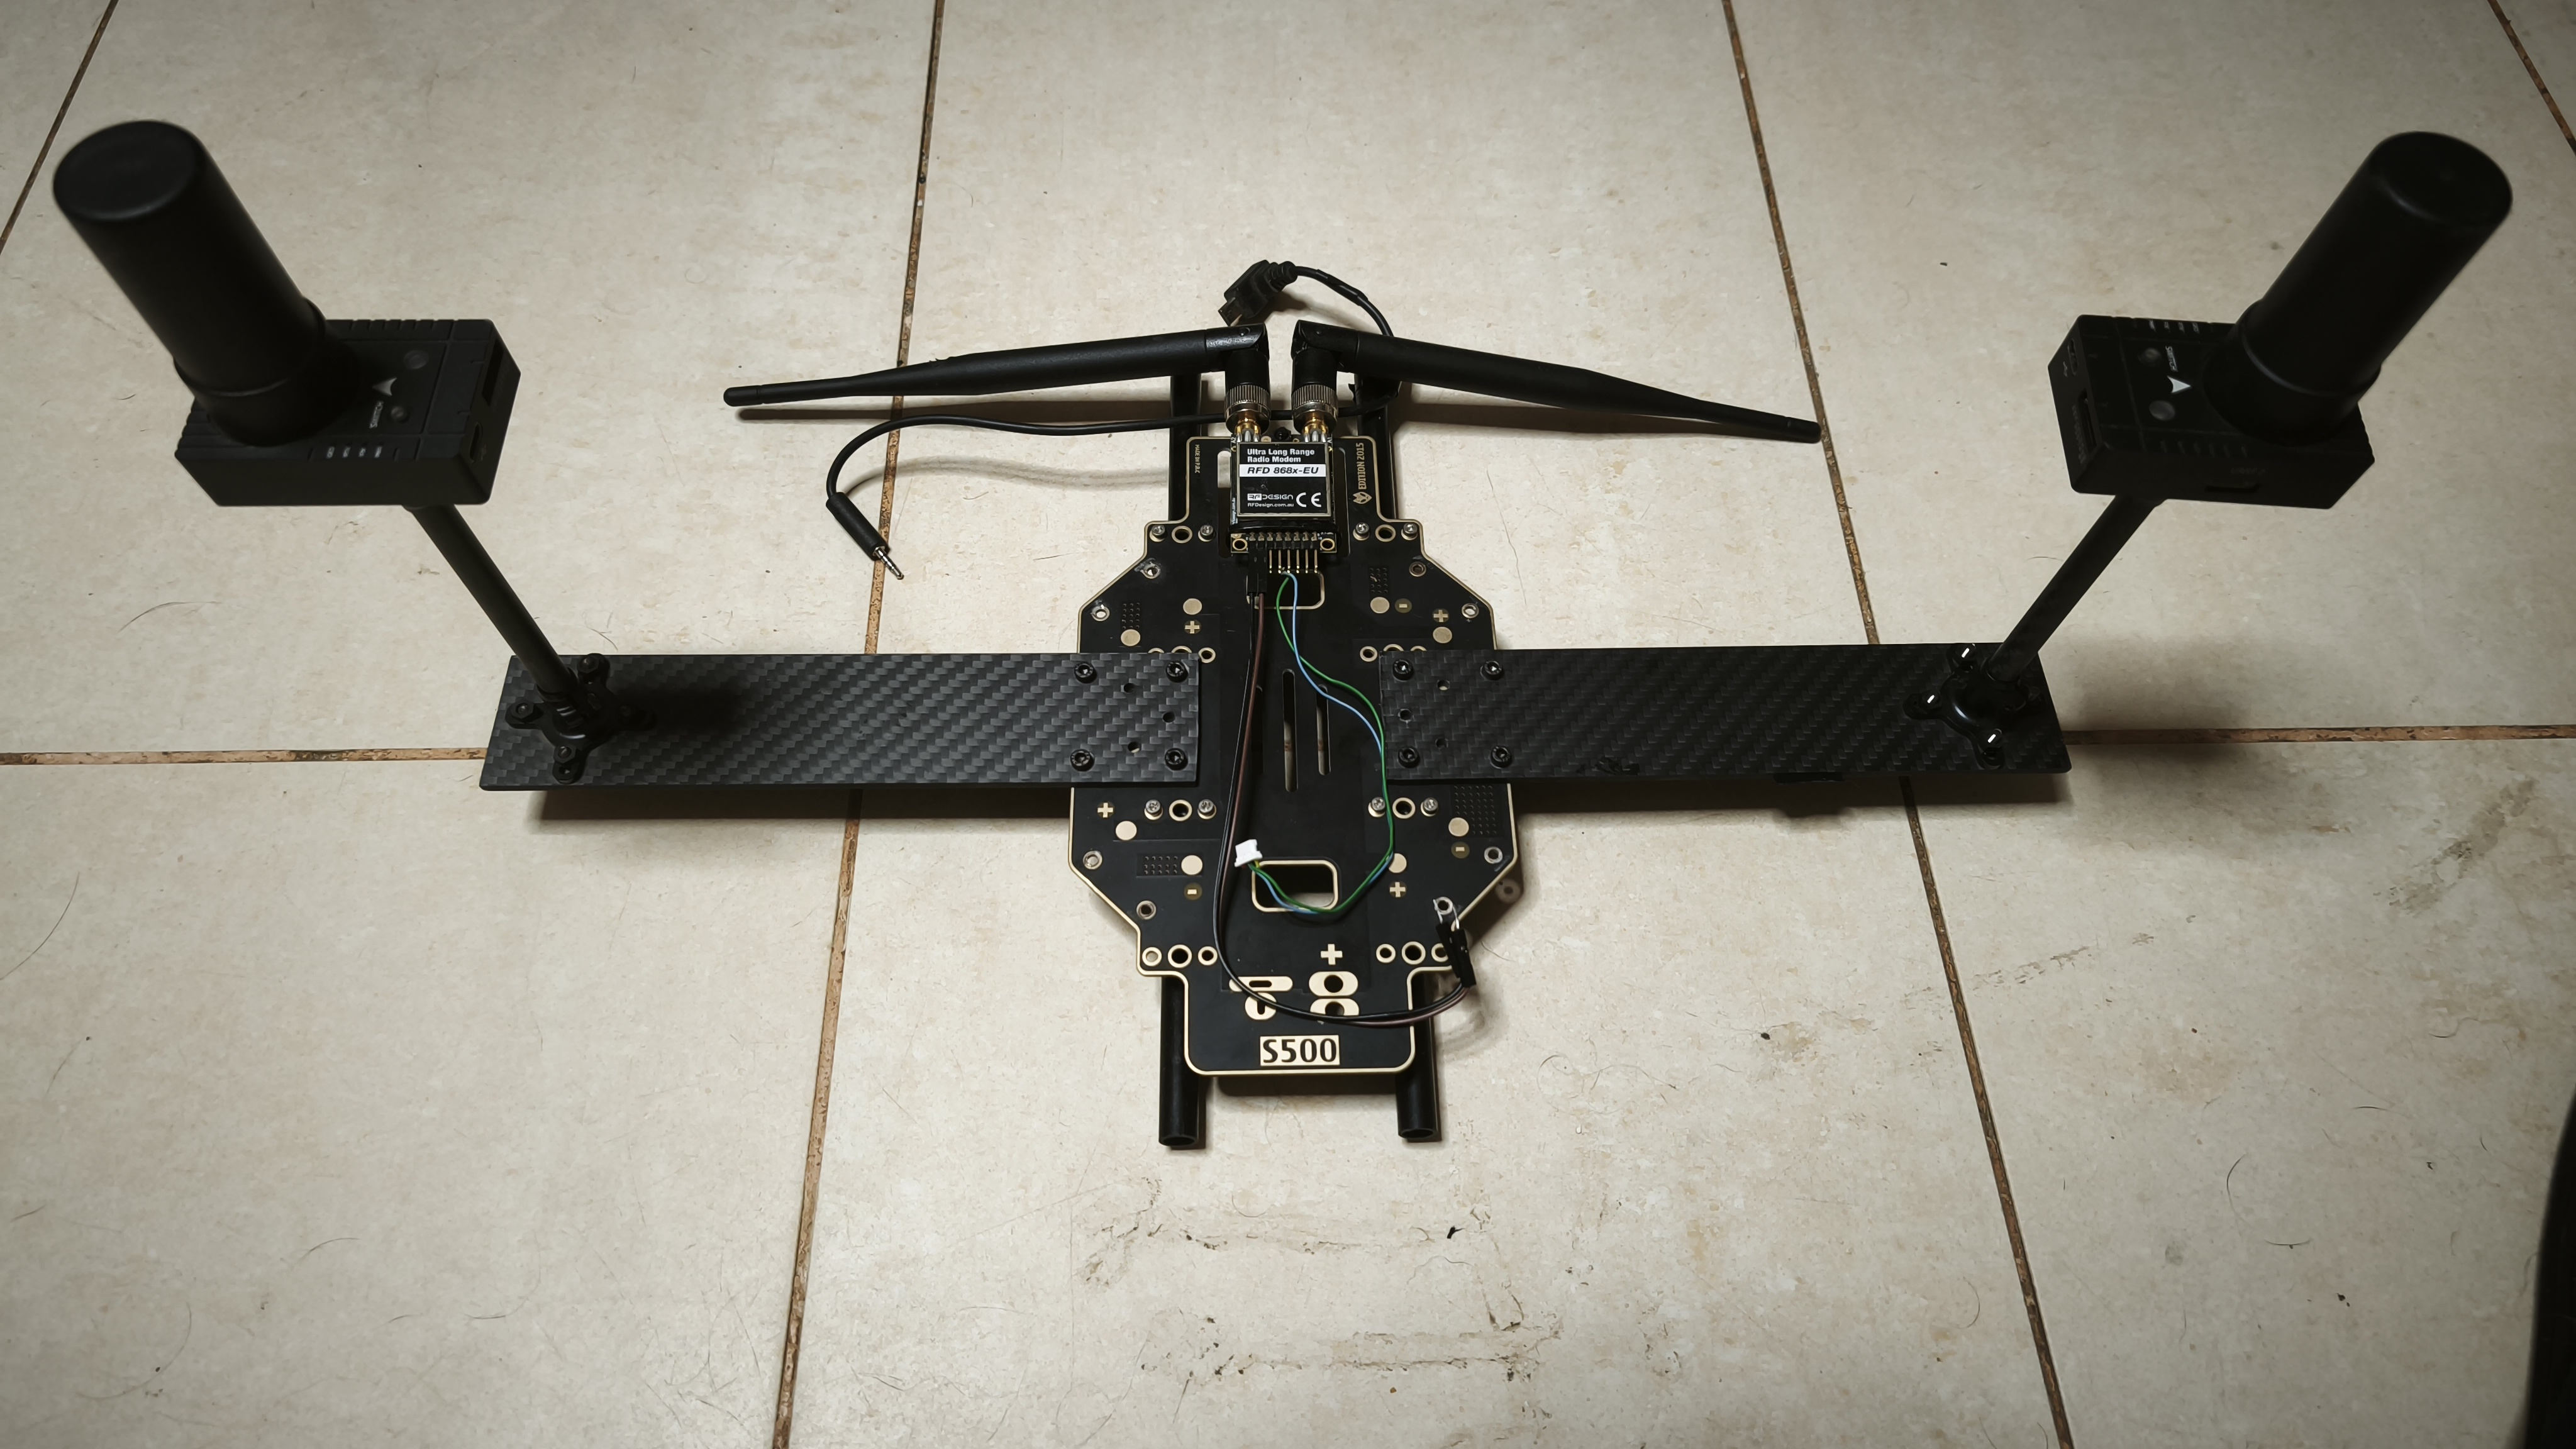
\includegraphics[width=\textwidth]{img/xasis_base.jpg}
    \caption{Placa central S500 amb el \emph{bracket} de carboni, els dos mòduls H-RTK F9P Helical sobre pals verticals i el mòdul RFD868x.}
    \label{fig:xassis-base}
\end{figure}

\begin{figure}[H]
    \centering
    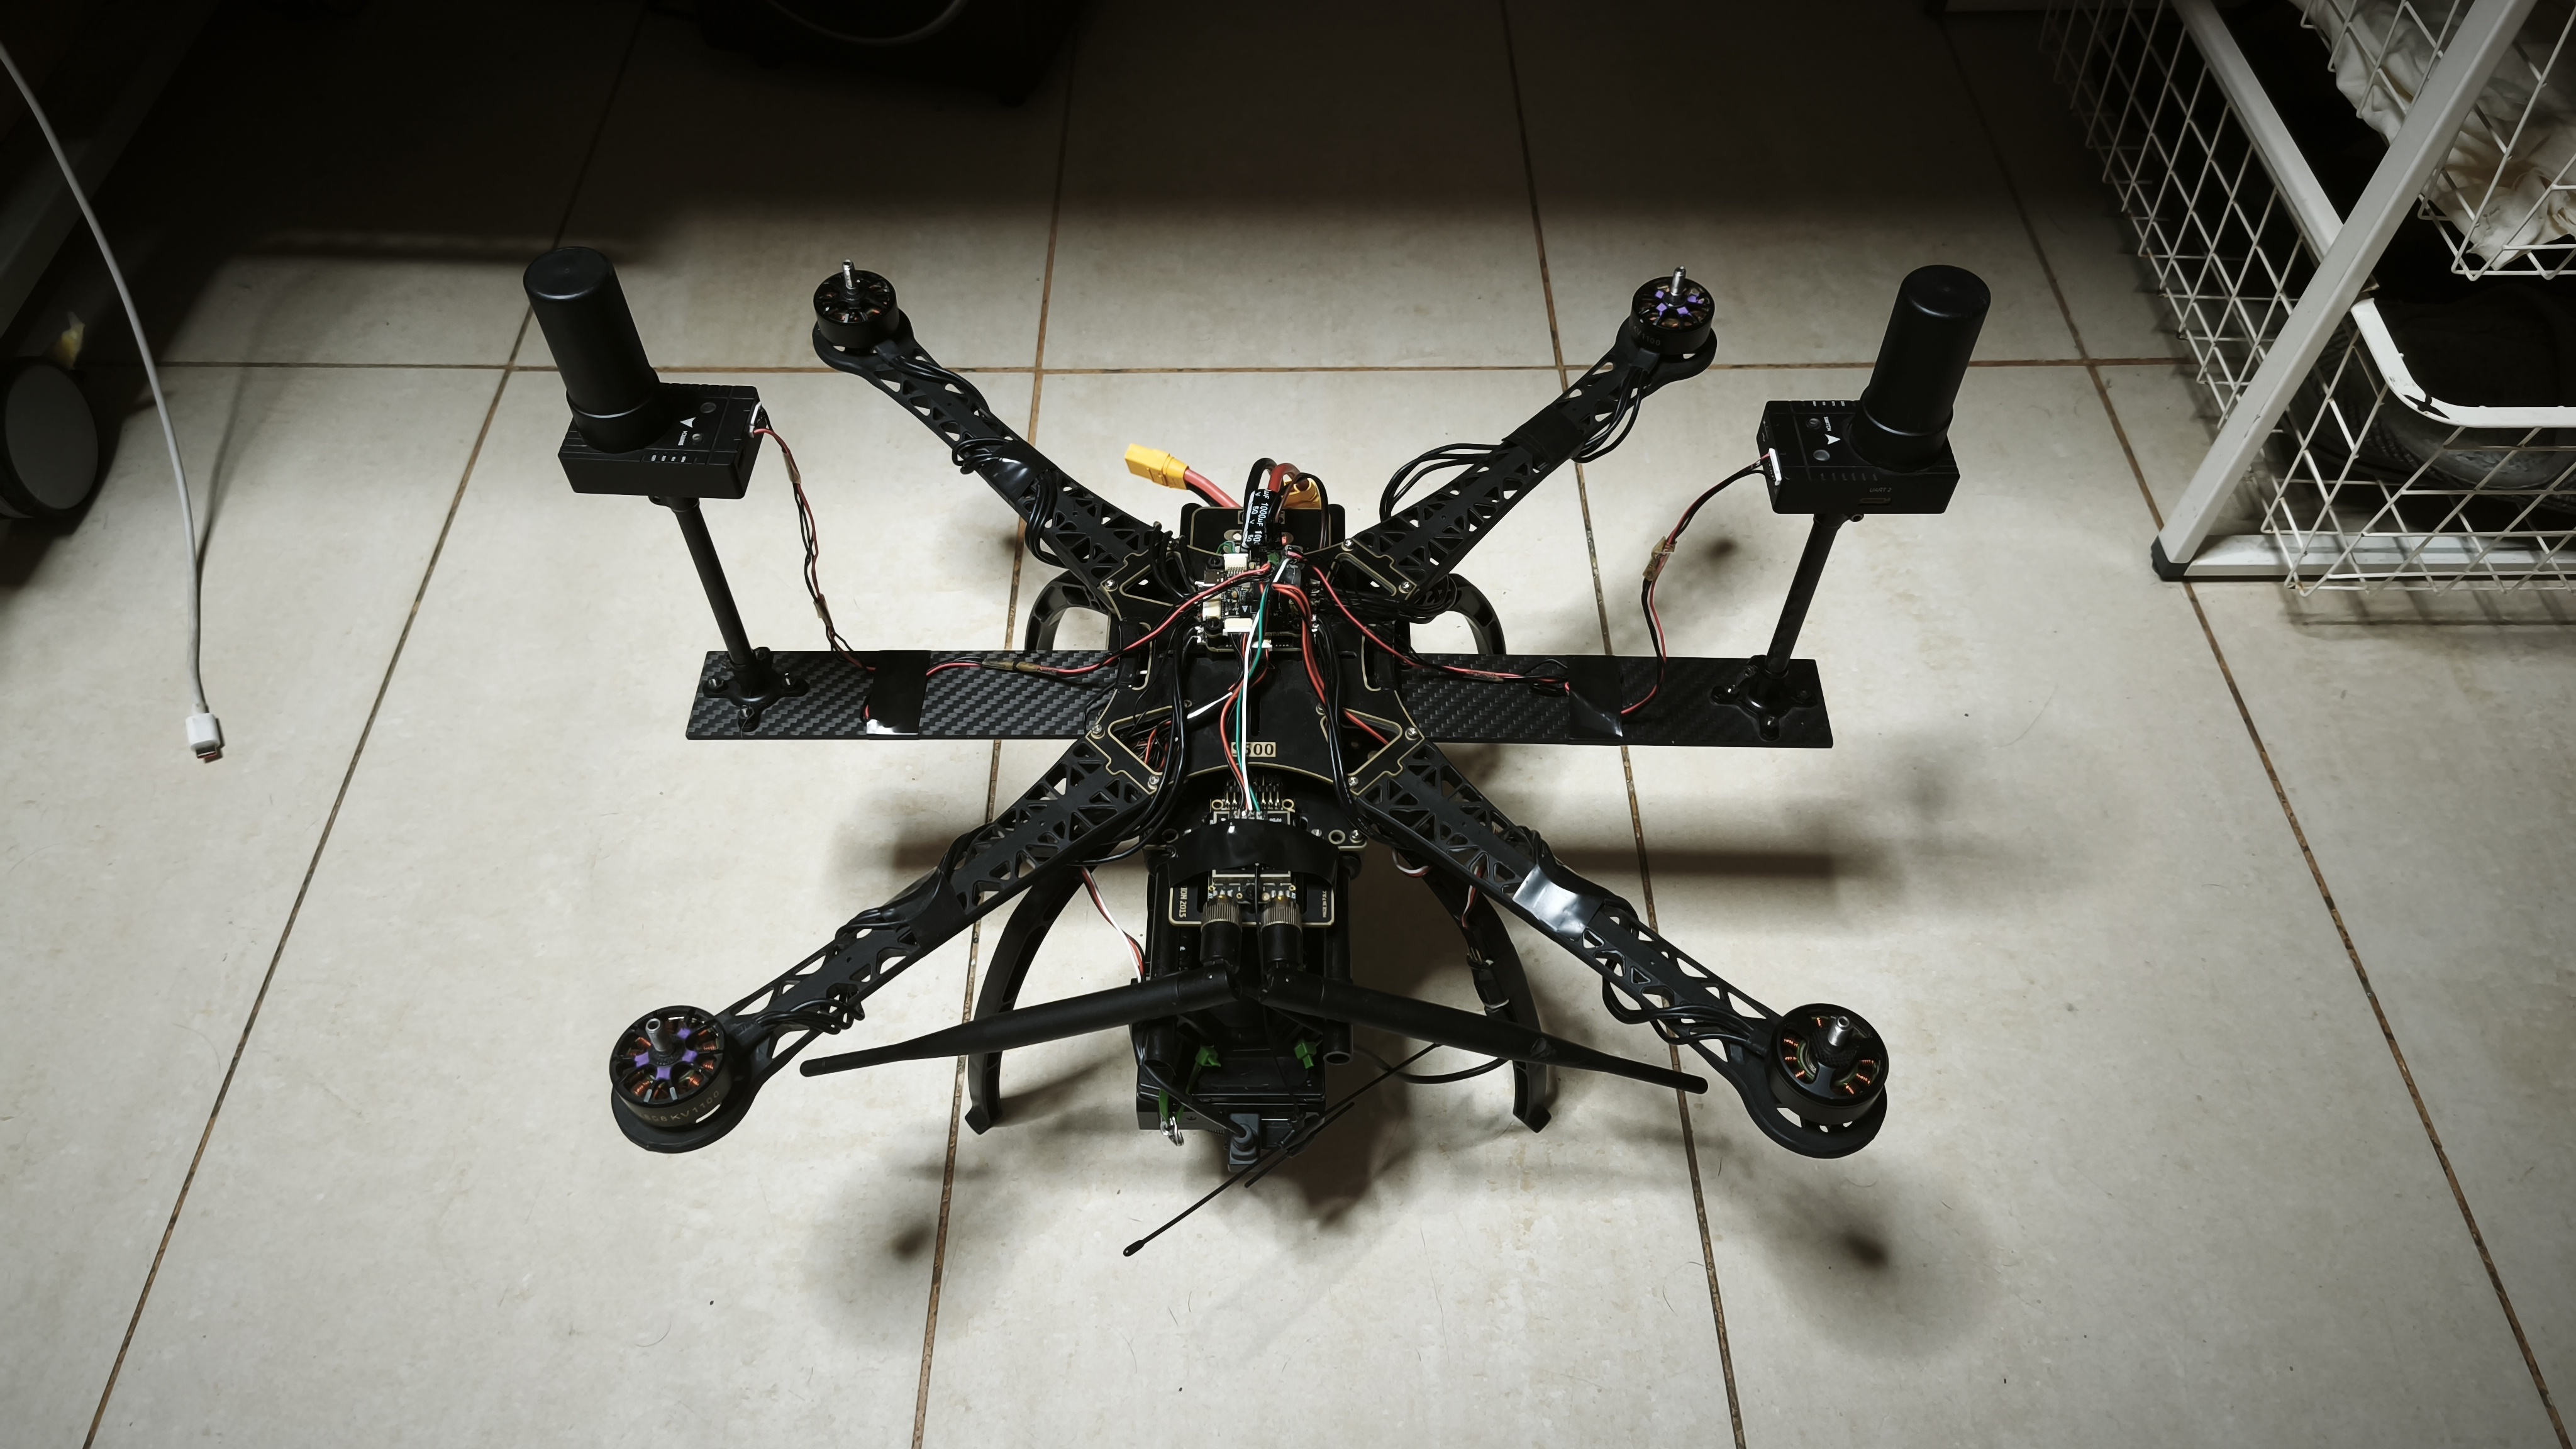
\includegraphics[width=\textwidth]{img/xasis_sencer.jpg}
    \caption{Dron acabat, vist des de dalt: motors, \emph{baseline} lateral amb les dues antenes GNSS, mòdul de telemetria i tren d'aterratge.}
    \label{fig:xassis-sencer}
\end{figure}

Sota el \emph{frame} hi ha un carril format per dues barres de carboni paral·leles amb abraçadores (\cref{fig:xassis-abaix}), que serveix de suport alhora per a la càmera i per a la bateria. La càmera (Sony $\alpha$6000 amb l'òptica de 25~mm) va a nadir, amb el Seagull SYNC2 a la sabata; la bateria 6S es subjecta al mateix carril, de manera que el centre de gravetat queda a prop de l'eix vertical del dron.

\begin{figure}[H]
    \centering
    \begin{subfigure}[b]{0.49\textwidth}
        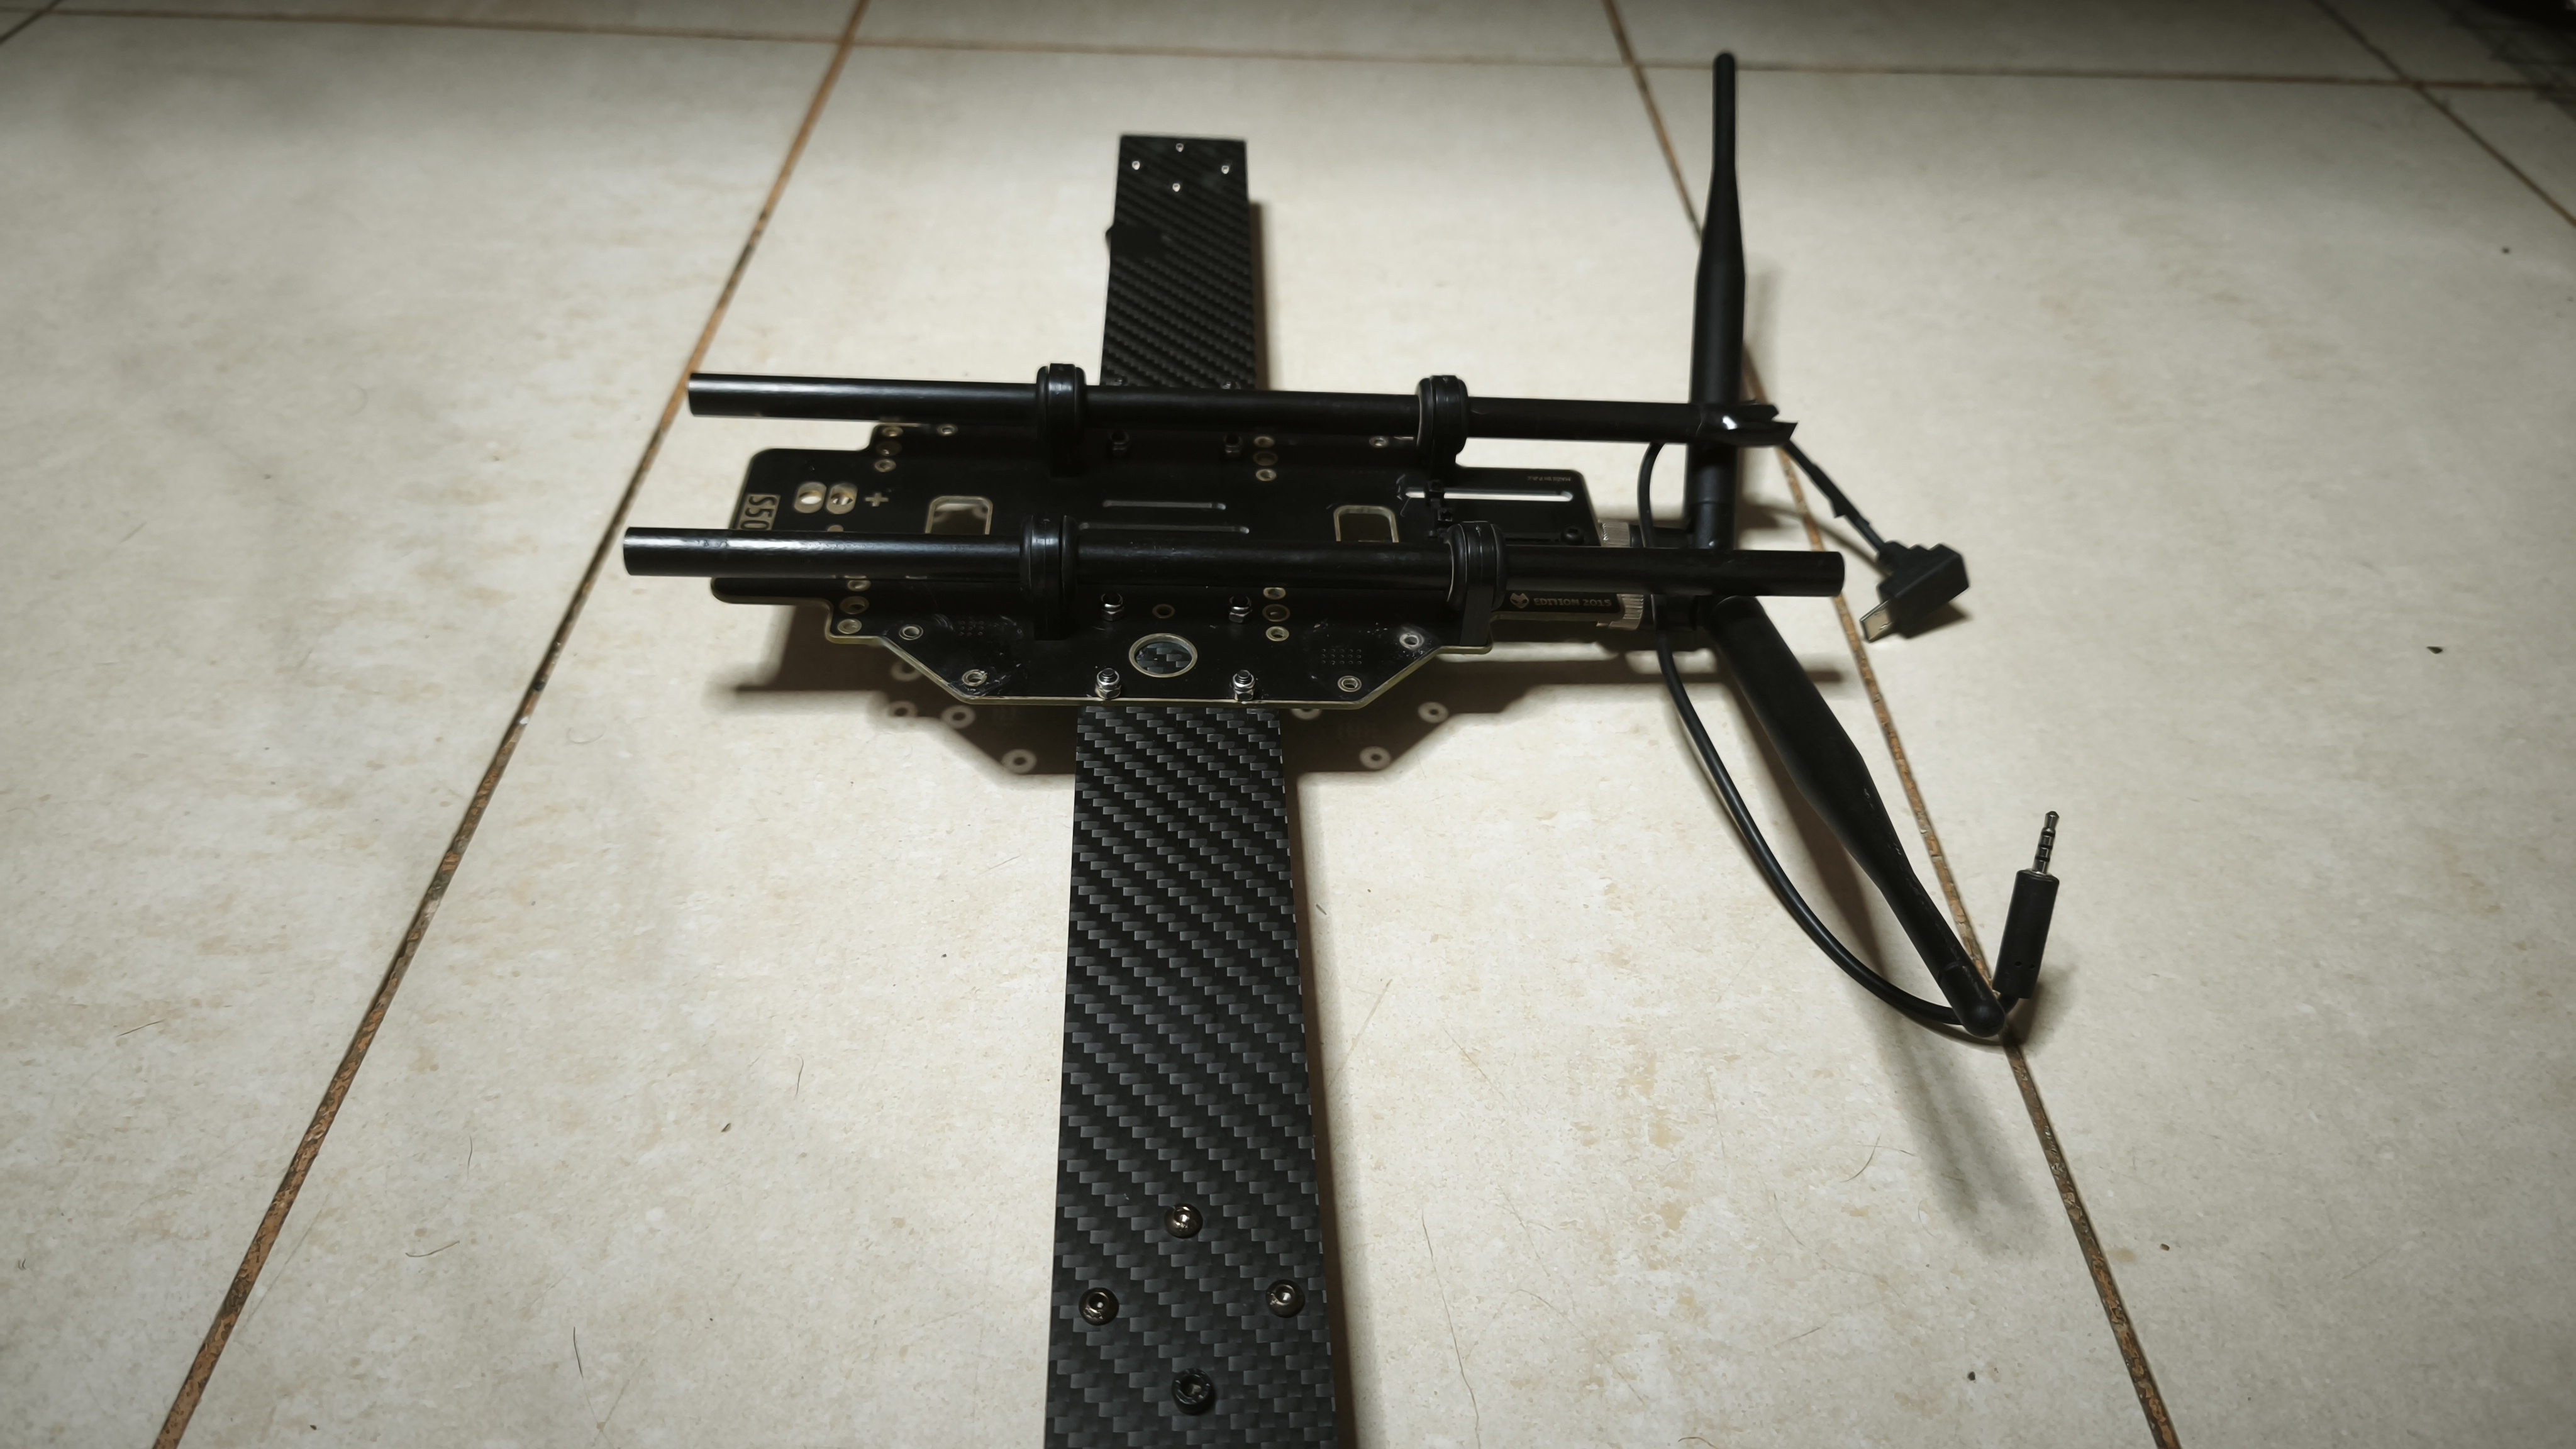
\includegraphics[width=\textwidth]{img/xasis_abaix_buit.jpg}
        \caption{Carril inferior sense càrrega.}
    \end{subfigure}
    \hfill
    \begin{subfigure}[b]{0.49\textwidth}
        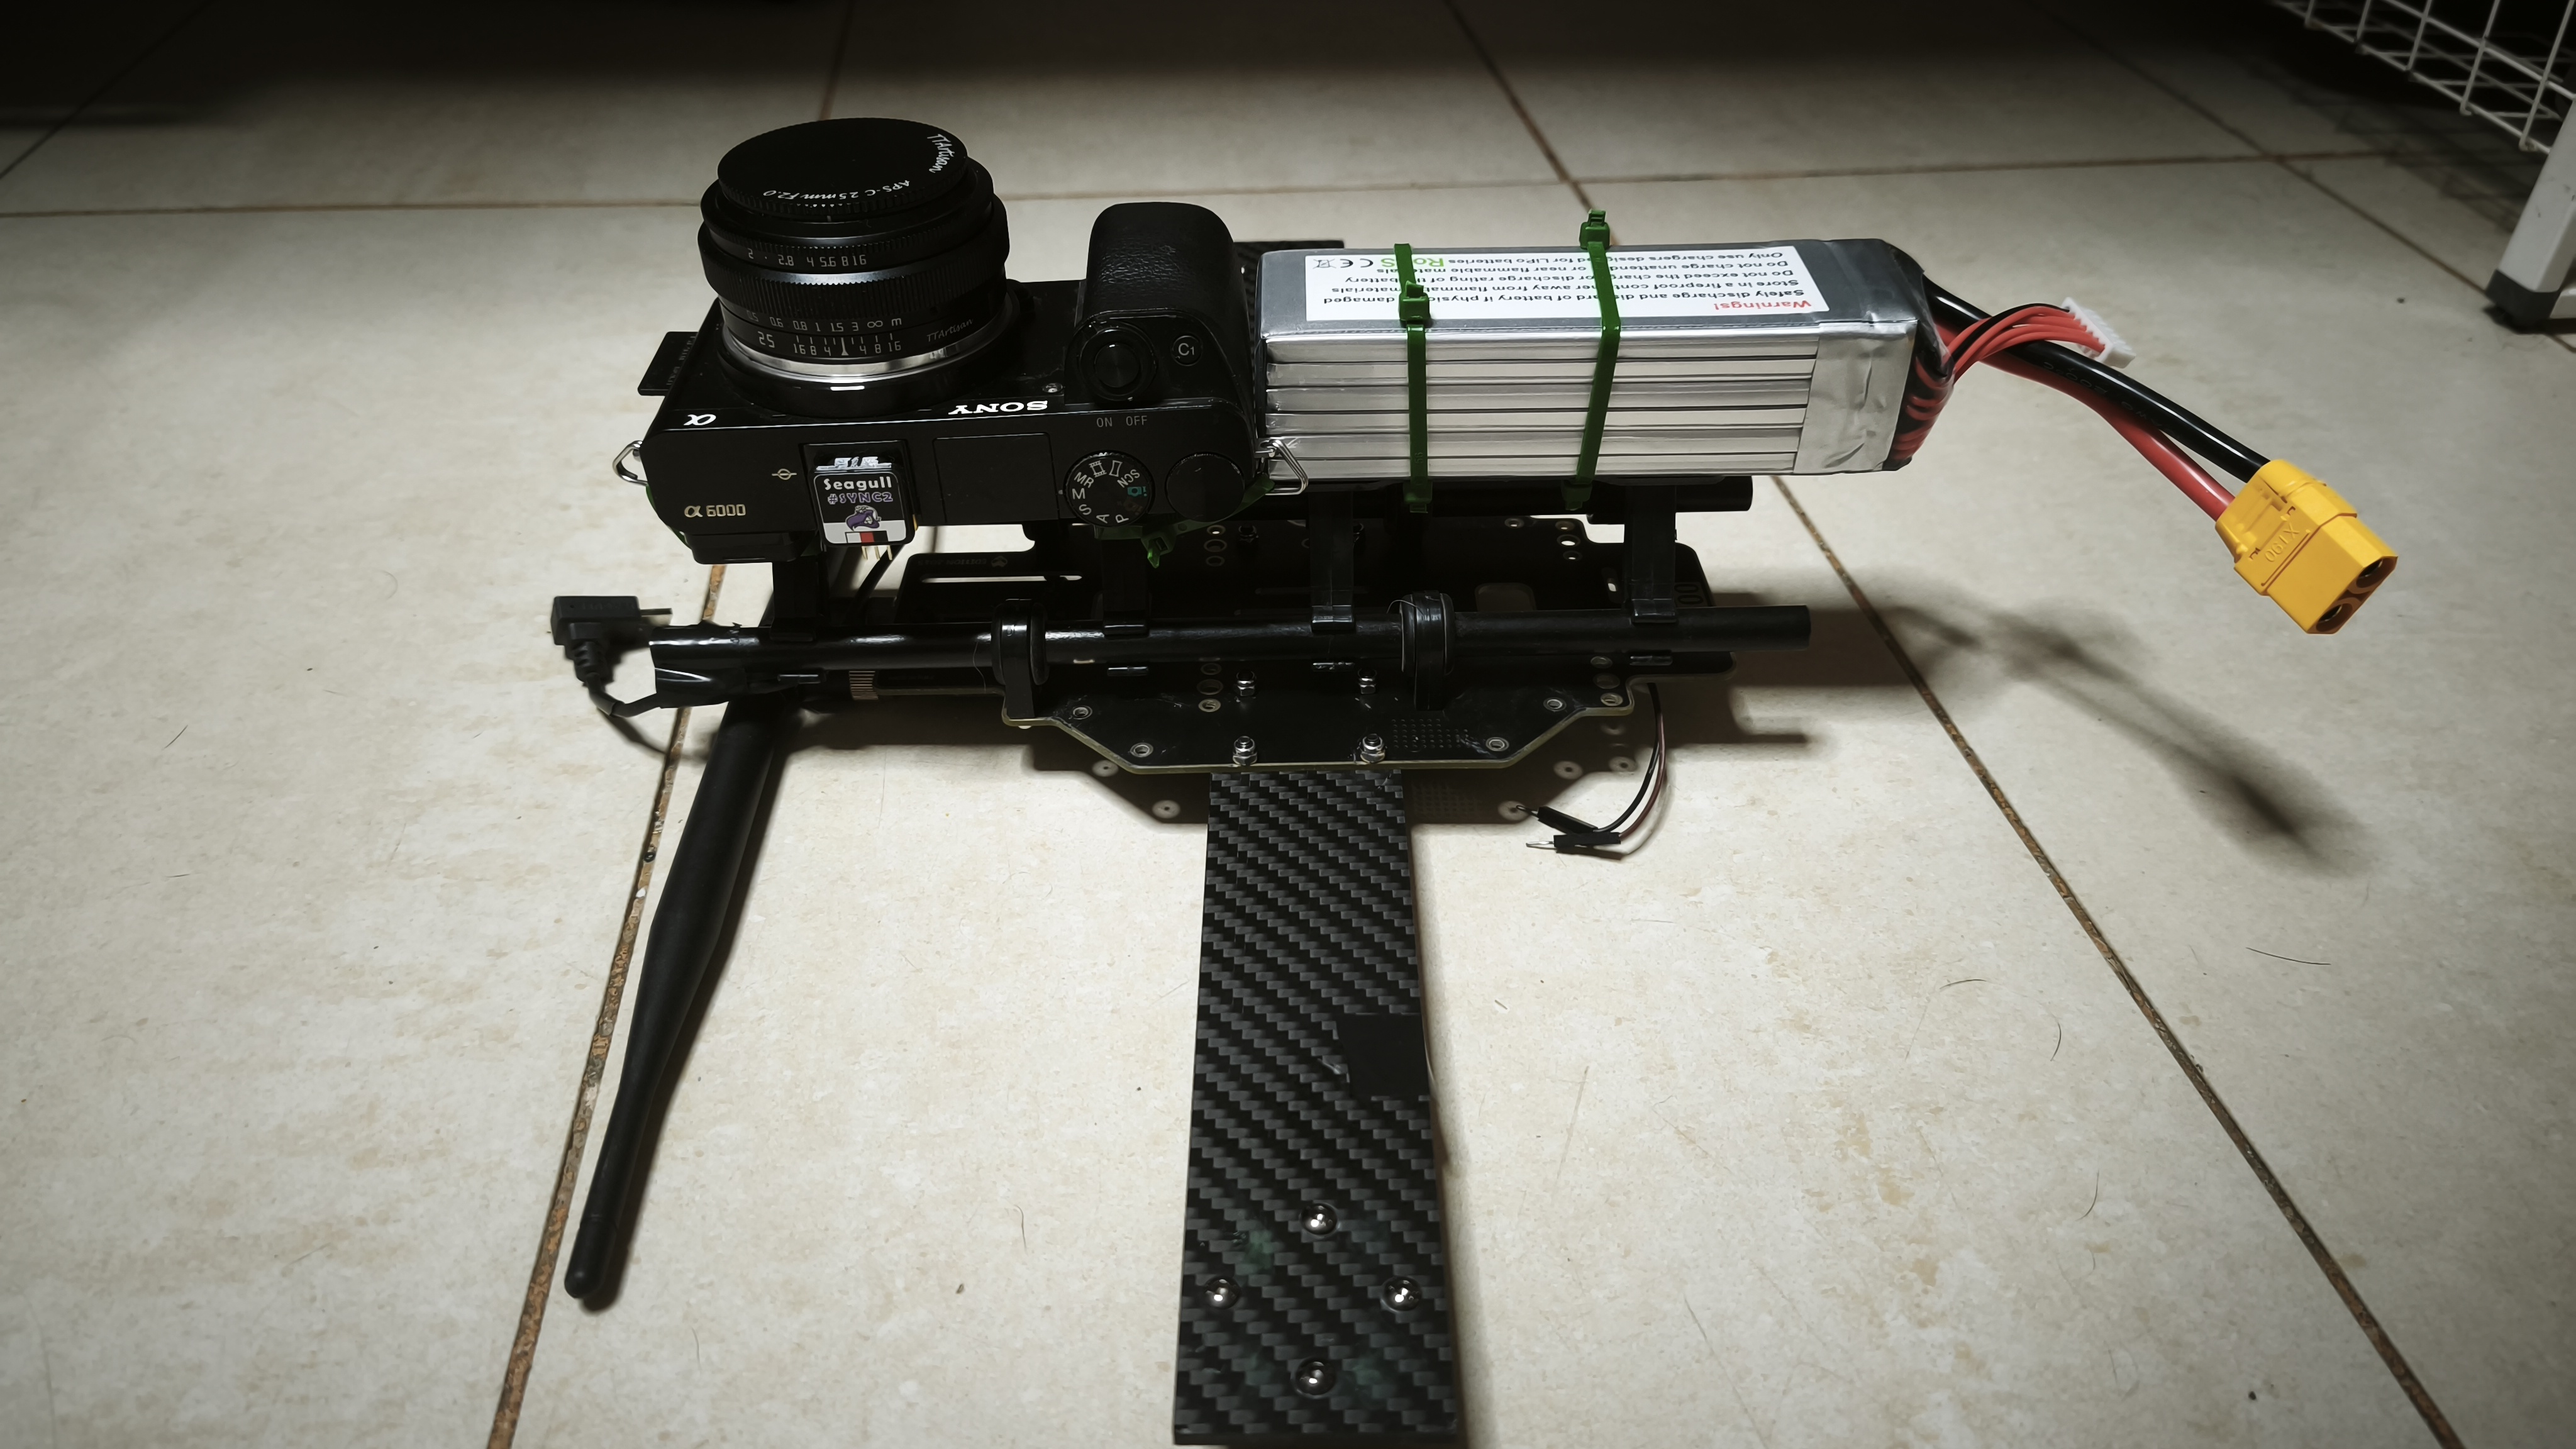
\includegraphics[width=\textwidth]{img/xasis_abaix_ple.jpg}
        \caption{Amb la càmera, el SYNC2 i la bateria.}
    \end{subfigure}
    \caption{Vista inferior del \emph{frame} (girat): carril de carboni i mòdul de càmera.}
    \label{fig:xassis-abaix}
\end{figure}

La configuració dels ports sèrie del FC i els paràmetres de \emph{firmware} (càmera, GPS \emph{moving baseline}) es descriuen al manual d'operació (\cref{chap:manual}).

\subsubsection*{Connexions elèctriques}

\Cref{fig:connexions} mostra el cablejat del dron i \cref{tab:connexions} el resumeix pad a pad. Tots els dispositius es connecten directament a pads del controlador de vol; cap receptor GNSS comparteix cable amb l'altre (el flux del \emph{moving baseline} passa pel controlador, \cref{subsec:gps-moving-baseline}).

\begin{figure}[p]
    \centering
    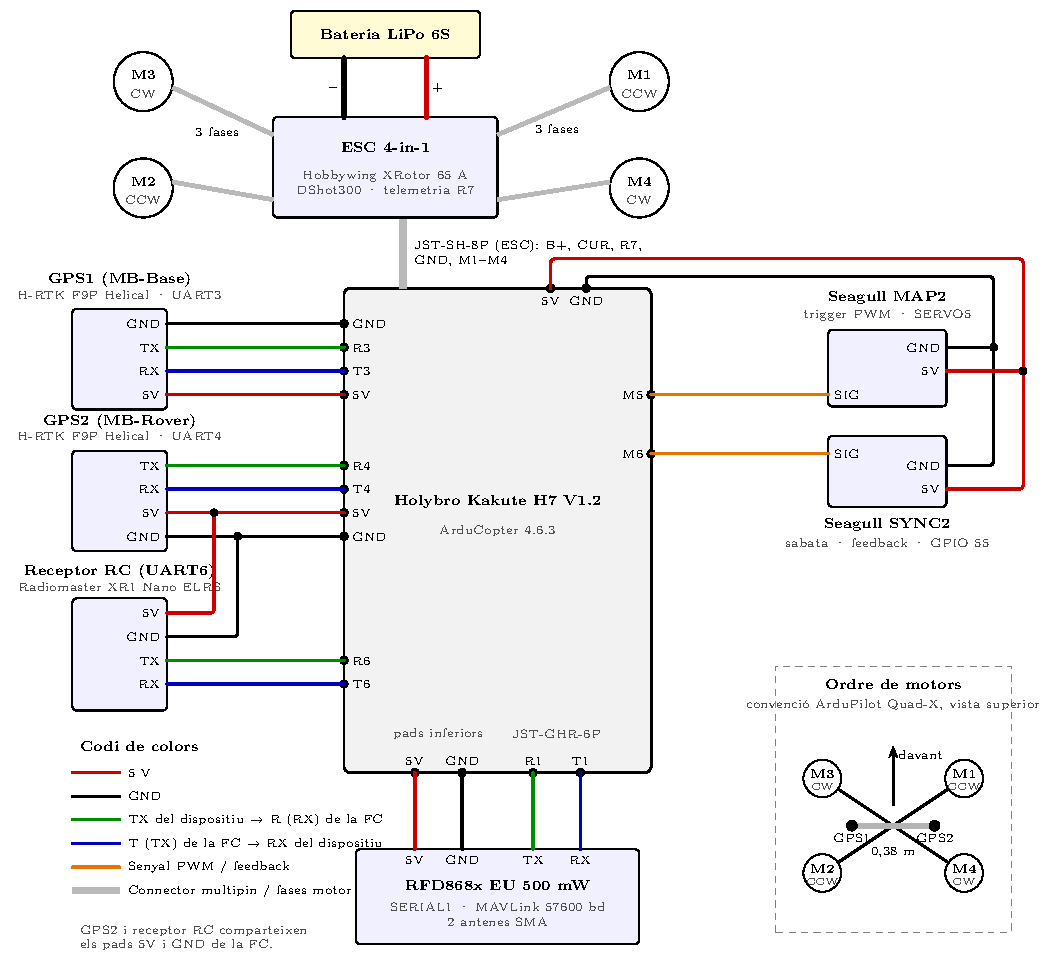
\includegraphics[width=\textwidth]{img/diagrama_connexions.pdf}
    \caption{Esquema de connexions del dron. Els colors segueixen el codi de la llegenda: verd per a la línia TX del dispositiu cap a l'RX de la FC i blau per a la TX de la FC cap a l'RX del dispositiu.}
    \label{fig:connexions}
\end{figure}

\begin{table}[H]
    \centering
    \caption{Connexions del controlador de vol (Kakute H7 V1.2)}
    \label{tab:connexions}
    \small
    \begin{tabular}{P{3.2cm}P{3.9cm}P{3.5cm}P{2.6cm}}
        \toprule
        Dispositiu & Pads de la FC & Funció & Port ArduPilot \\
        \midrule
        GPS1 (MB-Base) & R3, T3, 5V, GND & UART & \texttt{SERIAL3} \\
        GPS2 (MB-Rover) & R4, T4, 5V, GND & UART & \texttt{SERIAL4} \\
        Receptor ELRS & R6, T6, 5V, GND & UART (CRSF) & \texttt{SERIAL6} \\
        RFD868x & R1, T1 (JST-GHR-6P); 5V, GND & UART (MAVLink) & \texttt{SERIAL1} \\
        ESC 4-in-1 & JST-SH-8P: B+, CUR, R7, GND, M1--M4 & DShot, tensió, corrent, telemetria & \texttt{SERIAL7} \\
        Seagull MAP2 & M5; 5V, GND & PWM de \emph{trigger} & \texttt{SERVO5} \\
        Seagull SYNC2 & M6; 5V, GND & \emph{feedback} de la sabata & \texttt{SERVO6} (GPIO 55) \\
        \bottomrule
    \end{tabular}
\end{table}

\subsection{Base GNSS}
\label{subsec:muntatge-base}

La base és una pila compacta de tres plaques fixada a una pota del trípode amb brides (\cref{fig:base}): el receptor ArduSimple simpleRTK2B Pro (amb el ZED-F9P), la Raspberry Pi Zero W i el Waveshare UPS HAT amb les dues bateries 18650. L'antena BD900 GNSS es munta anivellada, amb pla de massa, sobre la rosca 5/8~polzades del trípode topogràfic, a una alçada de 122~cm als vols de prova.

Les connexions són (\cref{fig:base-connexions}):
\begin{itemize}
    \item \textbf{Antena $\rightarrow$ simpleRTK2B Pro:} cable coaxial amb connector SMA.
    \item \textbf{simpleRTK2B Pro $\rightarrow$ Raspberry Pi:} un cable USB-C, que porta les dades (correccions RTCM3 i configuració del receptor) i alimenta el receptor des de la Pi.
    \item \textbf{UPS HAT $\rightarrow$ Raspberry Pi:} només els pins de potència de la capçalera de la Pi es connecten al UPS HAT, que és qui l'alimenta amb les bateries; no hi ha cap línia de comunicació entre tots dos.
\end{itemize}

\begin{figure}[H]
    \centering
    \begin{tikzpicture}[box/.style={draw, rounded corners=2pt, align=center, font=\small, minimum height=10mm, minimum width=22mm, fill=blue!5},
        arr/.style={-{Stealth[length=2mm]}, thick}, node distance=17mm]
        \node[box] (ant) {Antena\\multibanda};
        \node[box, right=of ant] (rtk) {simpleRTK2B Pro\\(ZED-F9P)};
        \node[box, right=of rtk] (pi) {Raspberry Pi\\Zero W};
        \node[box, right=of pi] (ups) {UPS HAT\\2$\times$18650};
        \draw[arr] (ant) -- node[above, font=\scriptsize] {coaxial SMA} (rtk);
        \draw[arr] (rtk) -- node[above, font=\scriptsize] {USB-C} (pi);
        \draw[arr] (ups) -- node[above, font=\scriptsize] {pins 5~V} (pi);
    \end{tikzpicture}
    \caption{Connexions de la base RTK: antena, receptor, SBC i alimentació.}
    \label{fig:base-connexions}
\end{figure}

\begin{figure}[H]
    \centering
    \begin{subfigure}[b]{0.43\textwidth}
        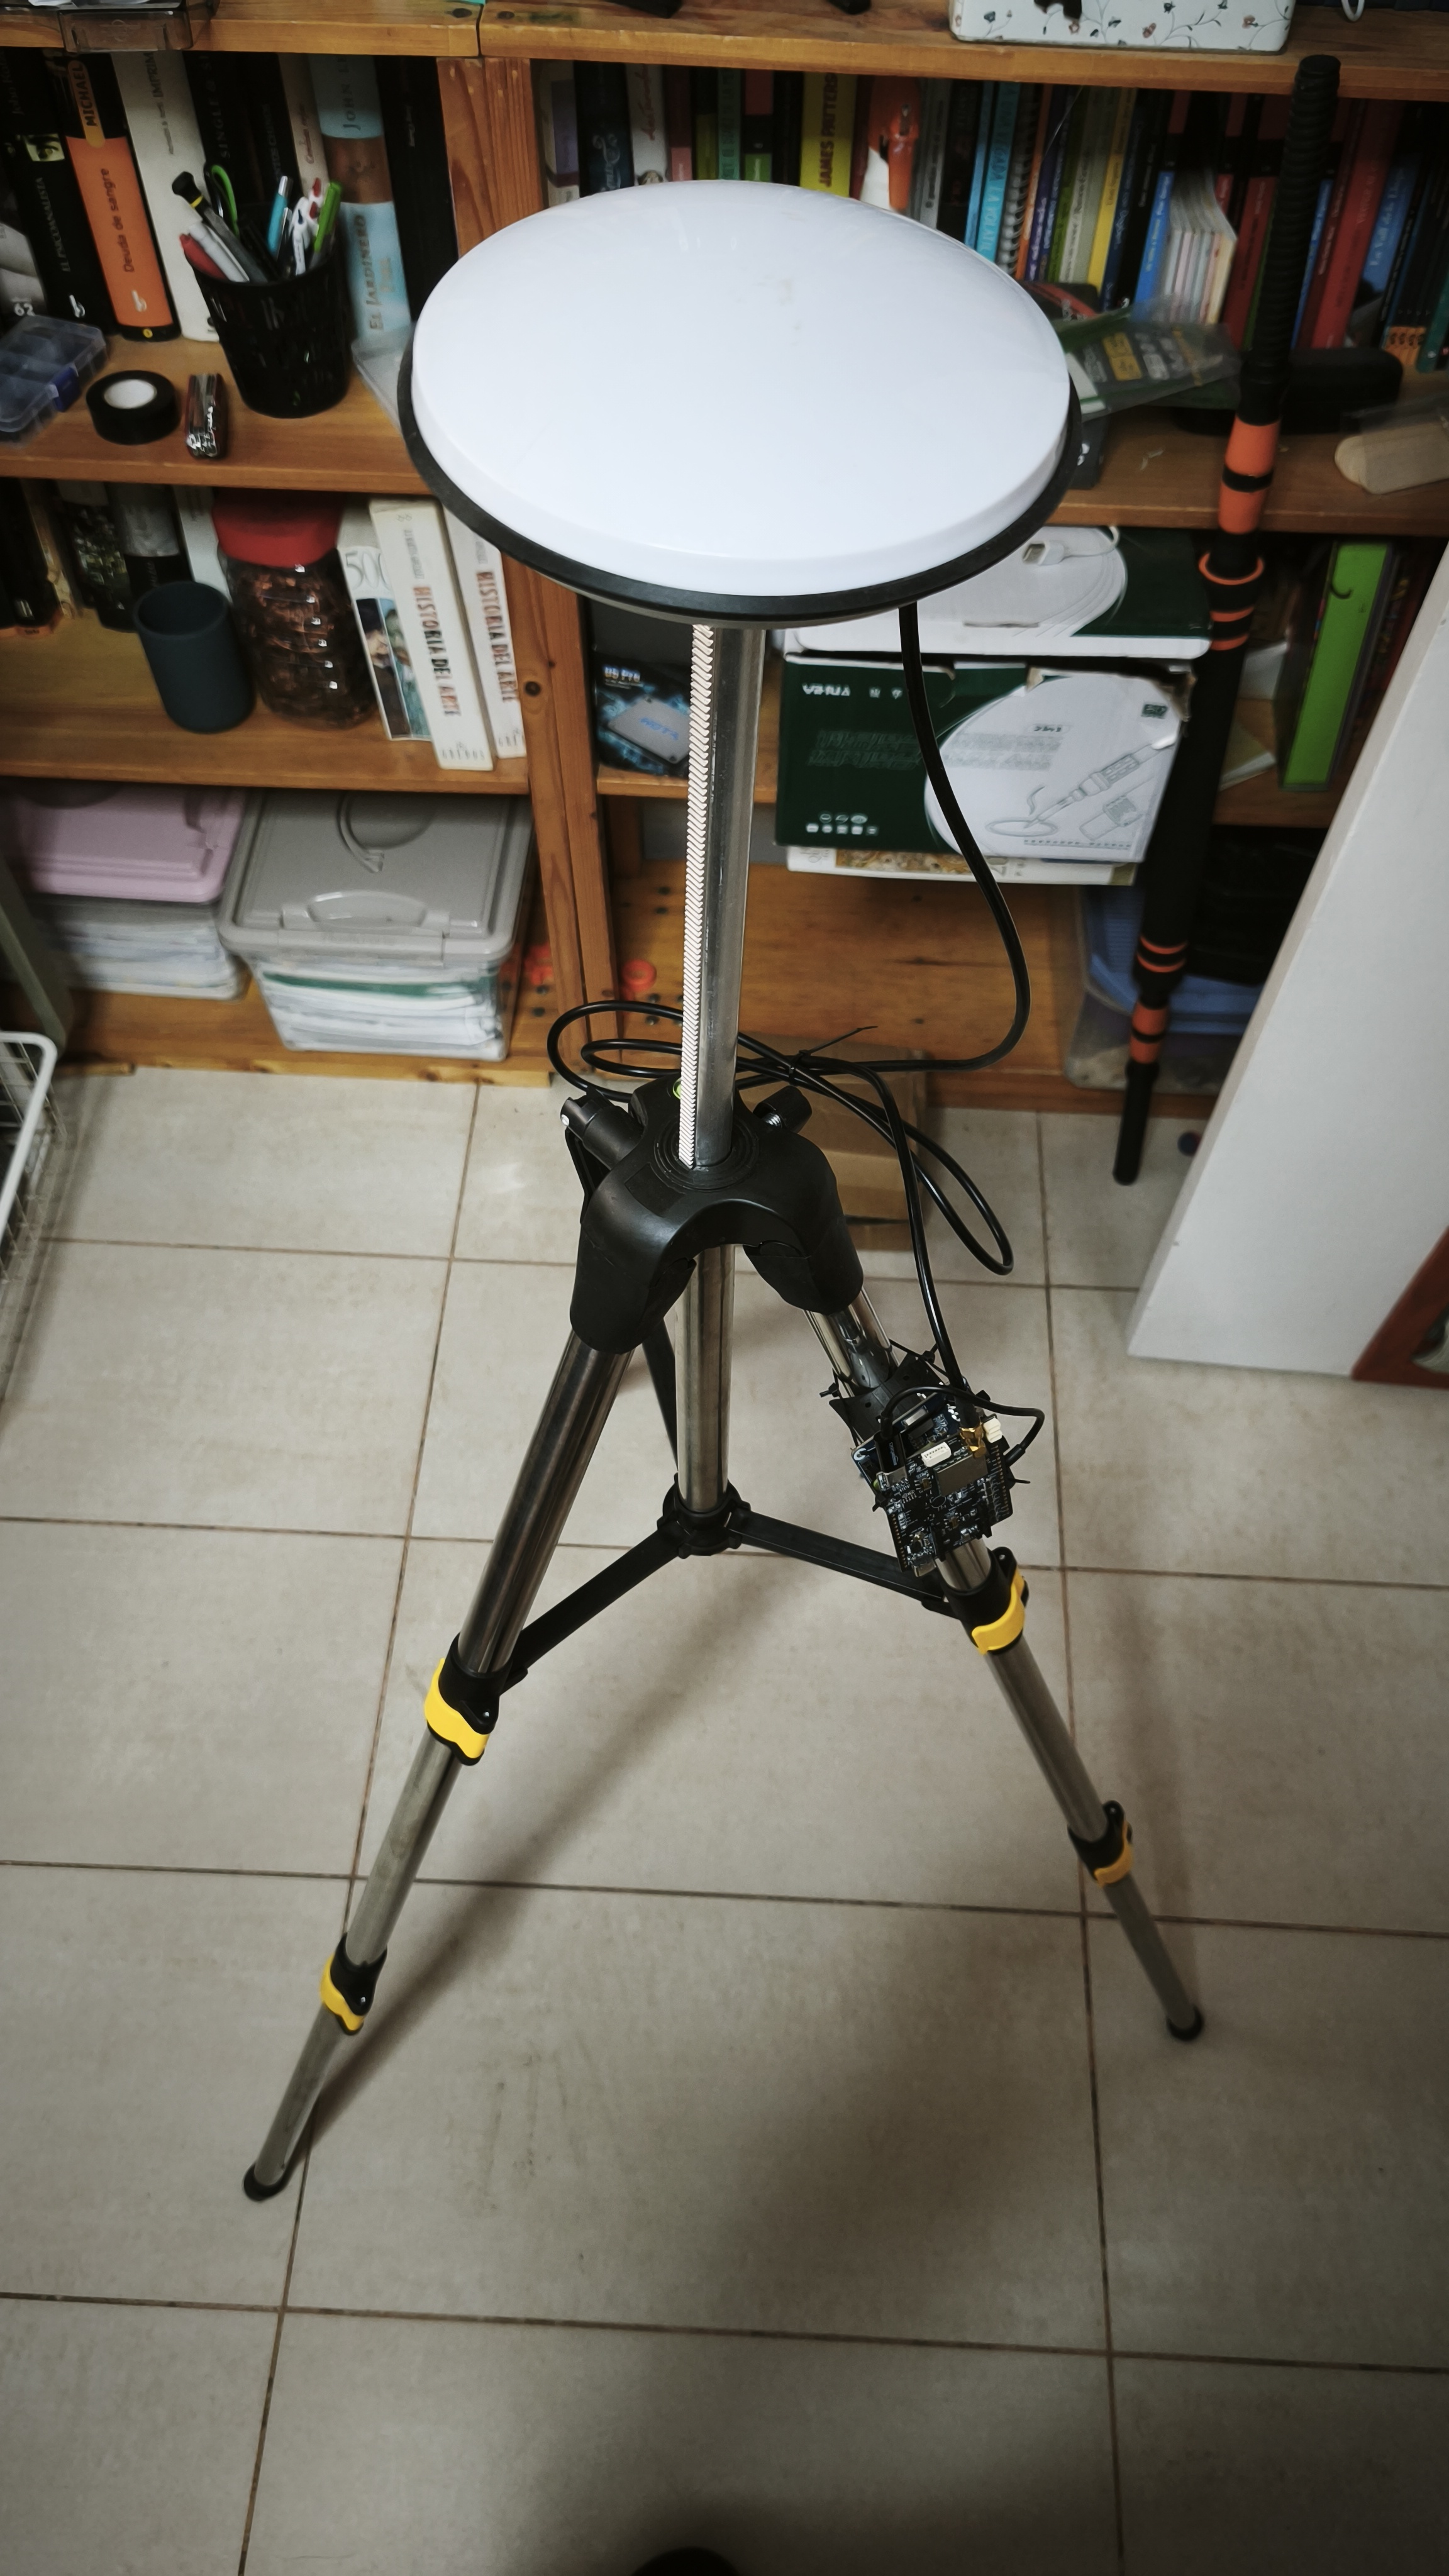
\includegraphics[width=\textwidth]{img/Base_sencera.jpg}
        \caption{Base completa sobre el trípode.}
    \end{subfigure}
    \hfill
    \begin{subfigure}[b]{0.43\textwidth}
        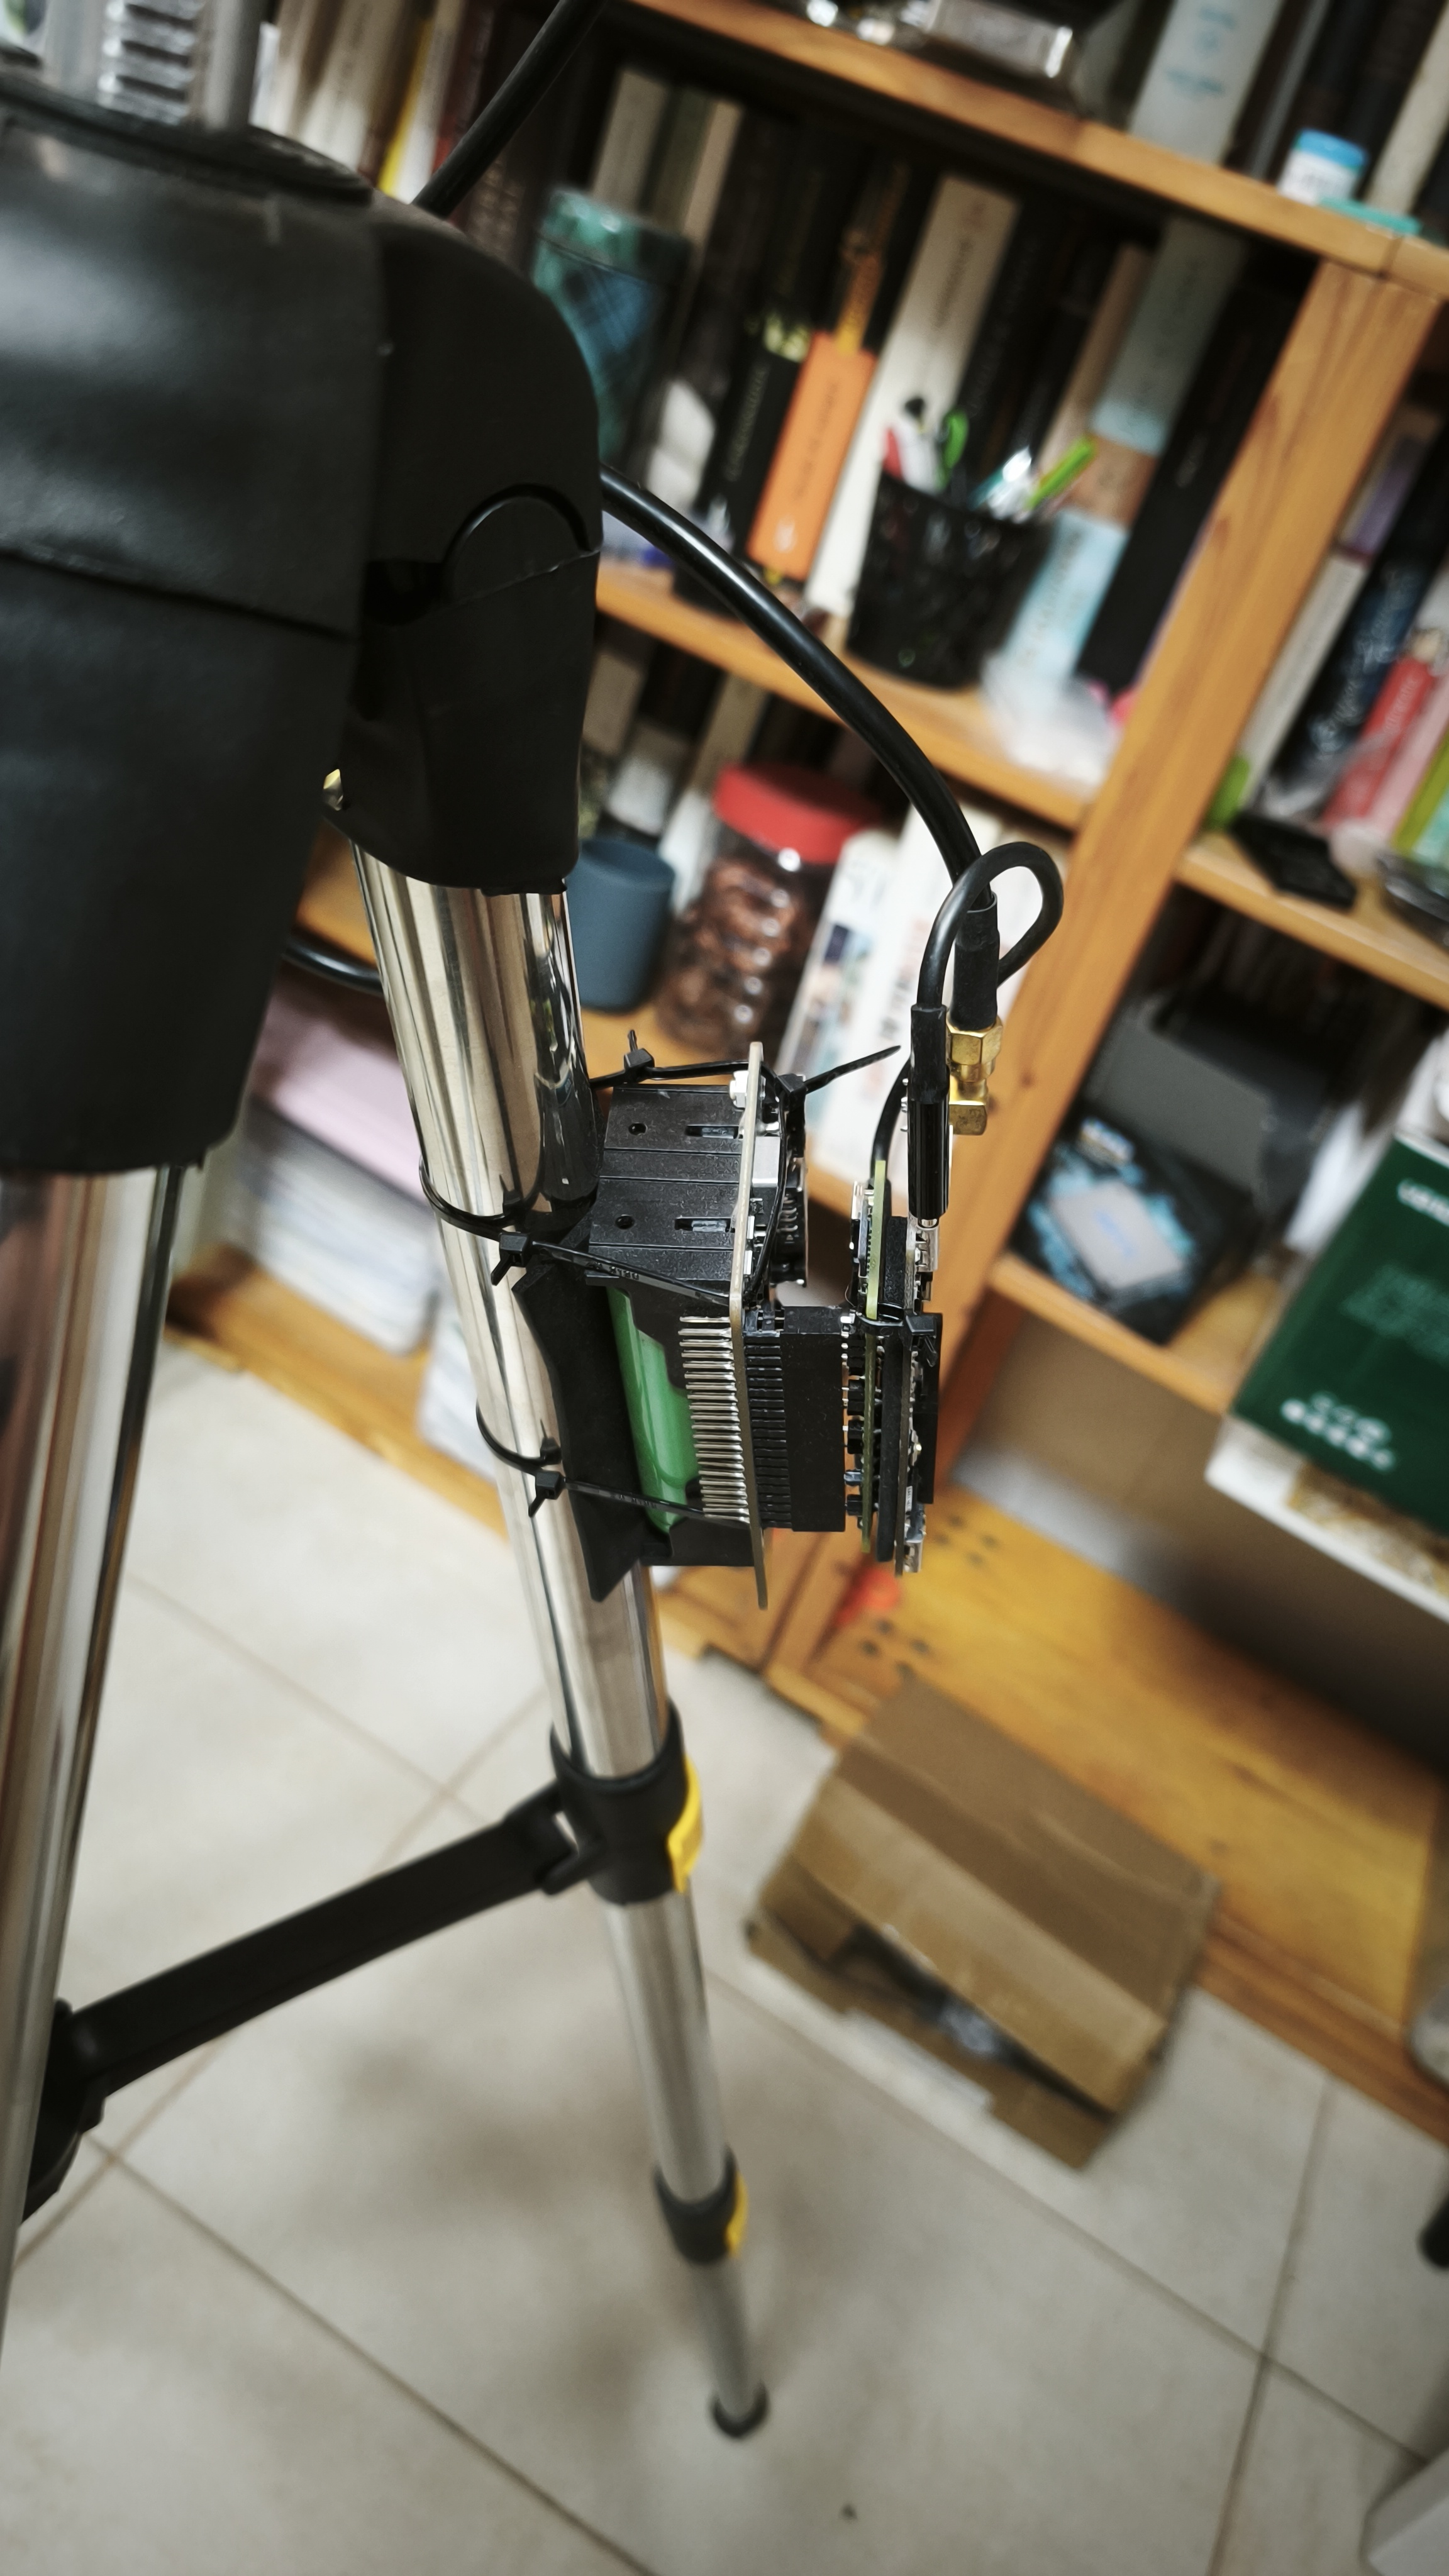
\includegraphics[width=\textwidth]{img/Stack_base.jpg}
        \caption{Pila de la base fixada a una pota.}
    \end{subfigure}
    \caption{Base RTK: antena multibanda sobre el trípode i pila amb el simpleRTK2B Pro, la Raspberry Pi i el UPS HAT.}
    \label{fig:base}
\end{figure}

El procediment de posicionament i de fixació de les coordenades de la base es descriu a \cref{sec:protocol-camp}.

\paragraph{Programari i configuració.} La Raspberry Pi funciona amb Raspberry Pi OS (Debian~13, 32~bits). Les correccions les distribueix el programa \texttt{str2str} de RTKLIB (la còpia \texttt{rtklibexplorer}, compilada a la pròpia Pi), executat com a servei \texttt{systemd} que arrenca amb la placa. El servei es diu \texttt{rtkbase}, però no té relació amb el projecte \texttt{rtkbase} de la bibliografia: llegeix el port sèrie USB del receptor (115\,200~bd) i obre un servidor TCP al port 5000 que reenvia el flux del receptor tal com surt (RTCM3 i els missatges UBX de navegació que emet pel mateix port), sense NTRIP. A més de reenviar-lo, el servei el desa a un fitxer durant tota la sessió (\cref{sec:protocol-camp}). La GS s'hi connecta amb \emph{RTK/GPS Inject} de Mission Planner en mode \emph{TCP Client}, a \texttt{192.168.4.1:5000}.

El punt d'accés WiFi (\texttt{BaseRTK}) el gestiona NetworkManager en mode \emph{shared}: banda de 2,4~GHz, canal~6, WPA-PSK, adreça \texttt{192.168.4.1/24} amb DHCP, i s'activa a cada arrencada. Cal desactivar el PMF (802.11w), perquè el controlador \texttt{brcmfmac} de la Pi no el suporta en mode AP.

El ZED-F9P (\emph{firmware} HPG~1.51, protocol~27.50) es configura amb \texttt{ubxtool}: NMEA desactivat al port USB, RTCM3 activat i els missatges 1005, 1074, 1084, 1094, 1124 i 1230 a 1~Hz. El flux total del port 5000, amb els missatges UBX de navegació que el receptor també emet, va ser d'uns 15~kbps. La posició de la base no es fixa: el receptor fa un \emph{survey-in} a cada sessió, amb 300~s com a mínim i fins que la precisió de la mitjana és de 2~m o millor, i la configuració queda guardada a la memòria \emph{flash} del receptor. Els vols de prova 5 i 6 van fer servir aquesta base i aquest mètode, amb l'antena a 122~cm.

\textbf{Limitació.} Als vols de prova 5 i 6 el servei només reenviava el flux, sense desar-lo, i no es va anotar la posició resultant del \emph{survey-in}; per això la posició absoluta d'aquells vols no es pot recuperar. Com que cada sessió en fa un de nou, la posició absoluta del mapa té un error comú de l'ordre de metres; això desplaça el mapa sencer però no en canvia la geometria relativa. Des del 27 d'octubre de 2026 el servei desa el flux de cada sessió, de manera que la posició es pot calcular a posteriori (\cref{sec:protocol-camp}).

\section{Estat del sistema}
\label{sec:estat-actual}

El maquinari està complet i el sistema ha acumulat uns 30~minuts de vol segons el comptador del controlador, repartits entre la campanya de posada a punt (\cref{chap:proves-vol}) i dos vols de fotogrametria (\cref{chap:vols-prova}). Amb la configuració actual el dron vola amb RTK Fixed als dos receptors i \emph{yaw} GNSS vàlid, i la cadena fotogràfica (dispar per distància, \emph{feedback} de la sabata, geoetiquetat i processat) està operativa de punta a punta. Les limitacions vigents --~sobretot l'autonomia i la validació absoluta amb punts de control~-- es recullen a \cref{sec:balanc-vols,sec:autonomia}, i el treball pendent és a \cref{sec:pendents-proves-vol}.
